\section{Introduction}

Parallel texts, mixed Fraktur-Antiqua printing, dictionaries, and library
catalogs are of particular interest to much Digital Humanities research
and often contain multiple scripts and semantic markup. With the
increased availability of Optical Character Recognition software at
least in part accessible to the determined DH scholar robust script and
text emphasis detection methods are of special importance for effective
digitization of these works.

\begin{wrapfigure}{l}{24cm}
	\includegraphics[width=\linewidth]{high.png}
	\captionof{figure}{Script recognition on French-Arabic sample page}
	\label{fig:high}
\end{wrapfigure}

State of the art neural sequence-to-sequence models have largely supplanted
older character-based methods for Optical Character Recognition. While neural
methods have generally higher accuracy and decreased requirements on training
data annotation depth, script and text emphasis detection approaches do not translate well to recent OCR engines.

\textbf{Bibliotheca Arabica} aims to gain new insights into Arabic literature from 1150
to 1850 CE by analysing the production, transmission, and reception of texts.
The basis of this research are \textbf{\textasciitilde 500, mostly
multilingual, library manuscript catalogs with extensive semantic
markup} in the form of text emphasis.

\subsection*{Related work}

Past approaches to segmentation-less multilingual OCR have focused on building
combined models capable of recognizing multiple
scripts~\cite{ul2013can}. The irregularity of early modern printing
and large number of typefaces result in \textbf{character accuracy below 95\%
for mixed-font models} even on mono-script texts \cite{springmann2016automatic},
necessitates menial training data acquisition and retraining of these
large models. Direct reuse of training data is also regularly prevented
by a mixture of wanted and undesirable scripts.

The method described in \cite{fujii2017sequence} labeling whole lines using a
recurrent neural network is inappropriate for many humanities texts
because of extensive intra-line script switching. \cite{ul2015sequence}
published a conceptually simpler approach without feature extraction
directly classifying character script using an LSTM network. A refined
version of the latter method is the basis of our script detection
system.

\section*{RNNs for Script and Emphasis Detection}

\subsection*{Script Detection}

The system treats script detection as a \textbf{segmentation-less sequence
classification} problem. Instead of unique output labels per grapheme, all \textbf{code
points of a particular script are assigned the same label} (figure
\ref{fig:transcription}) and the network is trained to generate the
correct sequence of script labels using the CTC loss
function~\cite{graves2006connectionist}. 
On the face CTC is unsuitable for this task, as it includes no mechanism to
ensure temporal alignment between graphemes in the input sequence and output
activations; fortunately the network's activations are fairly close to their
corresponding location in the input image. The output sequence is then
used to split the line into single-script runs that can be classified
with monoscriptual recognition models.

\begin{wrapfigure}{l}{30cm}
	\includegraphics[width=\linewidth]{transcription.png}
	\centering
	\captionof{figure}{Modified ground truth (top: original line, middle: transcription,\\ bottom: assigned script classes)}
	\label{fig:transcription}
\end{wrapfigure}

Script classes are derived from the Unicode script property in conjunction with
ISO 15924 identifiers. \textbf{Graphemes occuring in multiple scripts such as
numerals and punctuation are assigned a separate common class.} Merging these
during post-processing based on their surrounding script increases
classification robustness on non-body text such as page numbers and tables.
Classification of bidirectional text is supported by applying the Unicode BiDi
algorithm before script assignment.

Two additional post-processing steps are performed. First individual runs are
replaced by the whole line bounding box if only a single script remains after
common/inherited merging. A second step increases accuracy through a
user-supplied whitelist of allowed scripts, merging invalid runs into the
surrounding context after filtering for common confusions.

\subsection*{Emphasis Recognition}
\label{sec:emph}

\begin{wrapfigure}{r}{12cm}
	\center
	\vspace{1cm}
	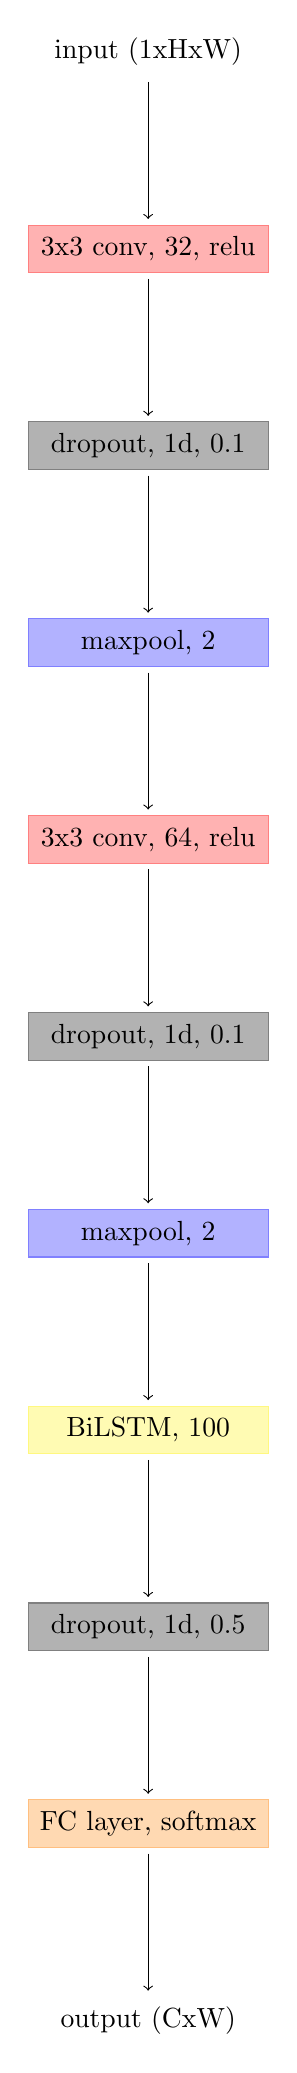
\begin{tikzpicture}[node distance = 2.5cm]
	\tikzset{
	  base/.style={draw, align=center, minimum height=4ex, rectangle, text centered},
	  proc/.style={base, draw=white, rectangle, text width=8em},
	  conv/.style={proc, draw=red!50, fill=red!30},
	  maxp/.style={proc, draw=blue!50, fill=blue!30},
	  drop/.style={proc, draw=black!50, fill=black!30},
	  lstm/.style={proc, draw=yellow!50, fill=yellow!30},
	  soft/.style={proc, draw=orange!50, fill=orange!30},
	  line/.style={draw, shorten <= 2pt, shorten >= 2pt, ->}
	}
	\node [proc] (input) {input (1xHxW)};
	\node [proc, conv, below of=input] (conv1) {3x3 conv, 32, relu};
	\node [proc, drop, below of=conv1] (drop1) {dropout, 1d, 0.1};
	\node [proc, maxp, below of=drop1] (maxp1) {maxpool, 2};
	\node [proc, conv, below of=maxp1] (conv2) {3x3 conv, 64, relu};
	\node [proc, drop, below of=conv2] (drop2) {dropout, 1d, 0.1};
	\node [proc, maxp, below of=drop2] (maxp2) {maxpool, 2};
	\node [proc, lstm, below of=maxp2] (lstm1) {BiLSTM, 100};
	\node [proc, drop, below of=lstm1] (drop3) {dropout, 1d, 0.5};
	\node [proc, soft, below of=drop3] (softm) {FC layer, softmax};
	\node [proc, below of=softm] (output) {output (CxW)};

	\path [line] (input) -- (conv1);
	\path [line] (conv1) -- (drop1);
	\path [line] (drop1) -- (maxp1);
	\path [line] (maxp1) -- (conv2);
	\path [line] (conv2) -- (drop2);
	\path [line] (drop2) -- (maxp2);
	\path [line] (maxp2) -- (lstm1);
	\path [line] (lstm1) -- (drop3);
	\path [line] (drop3) -- (softm);
	\path [line] (softm) -- (output);

	\end{tikzpicture}
	\captionof{figure}{Network architecture ($H$: sequence height, $W$: sequence length, $C$: alphabet size)}
	\label{fig:arch}
\end{wrapfigure}

We evaluated two methods of encoding two common text emphasis methods for
recognition by a neural network. Initially, \textbf{italicized and text components with
increased letter spacing} were marked up with special \textbf{start and stop markers}.
While the results of the training were promising, obtaining the amount of
training data needed to get the network to reliably place both markers was
infeasible for our target documents. Creating \textbf{separate labels for
italicized/spaced graphemes} and training for these, remedied the marker
placement issue with a sufficiently small amount of training data.

\subsection*{Architecture}

Both the script detection and emphasis recognition share a common network
architecture of a small \textbf{convolutional block followed by a bidirectional LSTM
layer} and a final linear projection with softmax activation as shown in figure
\ref{fig:arch}. The network is trained with \textbf{CTC loss and single-sample
stochastic gradient descent with momentum} (learning rate: 0.0001, momentum:
0.9). \textbf{Early stopping} is used to terminate training. The system is implemented
as part of the kraken OCR engine.

The networks operate on binarized whole lines. \textbf{Baselines and line height are
normalized} using a slightly modified version of the centerline normalizer
implemented in the OCRopus system. Labels and locations are extracted from the
$C\times W$ output matrix with a simple \textbf{greedy decoder}. 

\section*{Results}

\subsection*{Dataset}

We repurposed publicly available non-synthetic training data for recognition
models to build a corpus of \textbf{85000} script-annotated line images containing
\textbf{Arabic, Cyrillic, polytonic Greek, Hebrew, Latin, Fraktur, and (western) Syriac}
text. The majority of text lines contain only a single non-common script
although there are mixed lines for all scripts in the corpus. The exact
distribution of code points is shown in table \ref{table:points}. 850 randomly
selected lines are separated from the corpus as a test set.

\begin{wrapfigure}{l}{20cm}
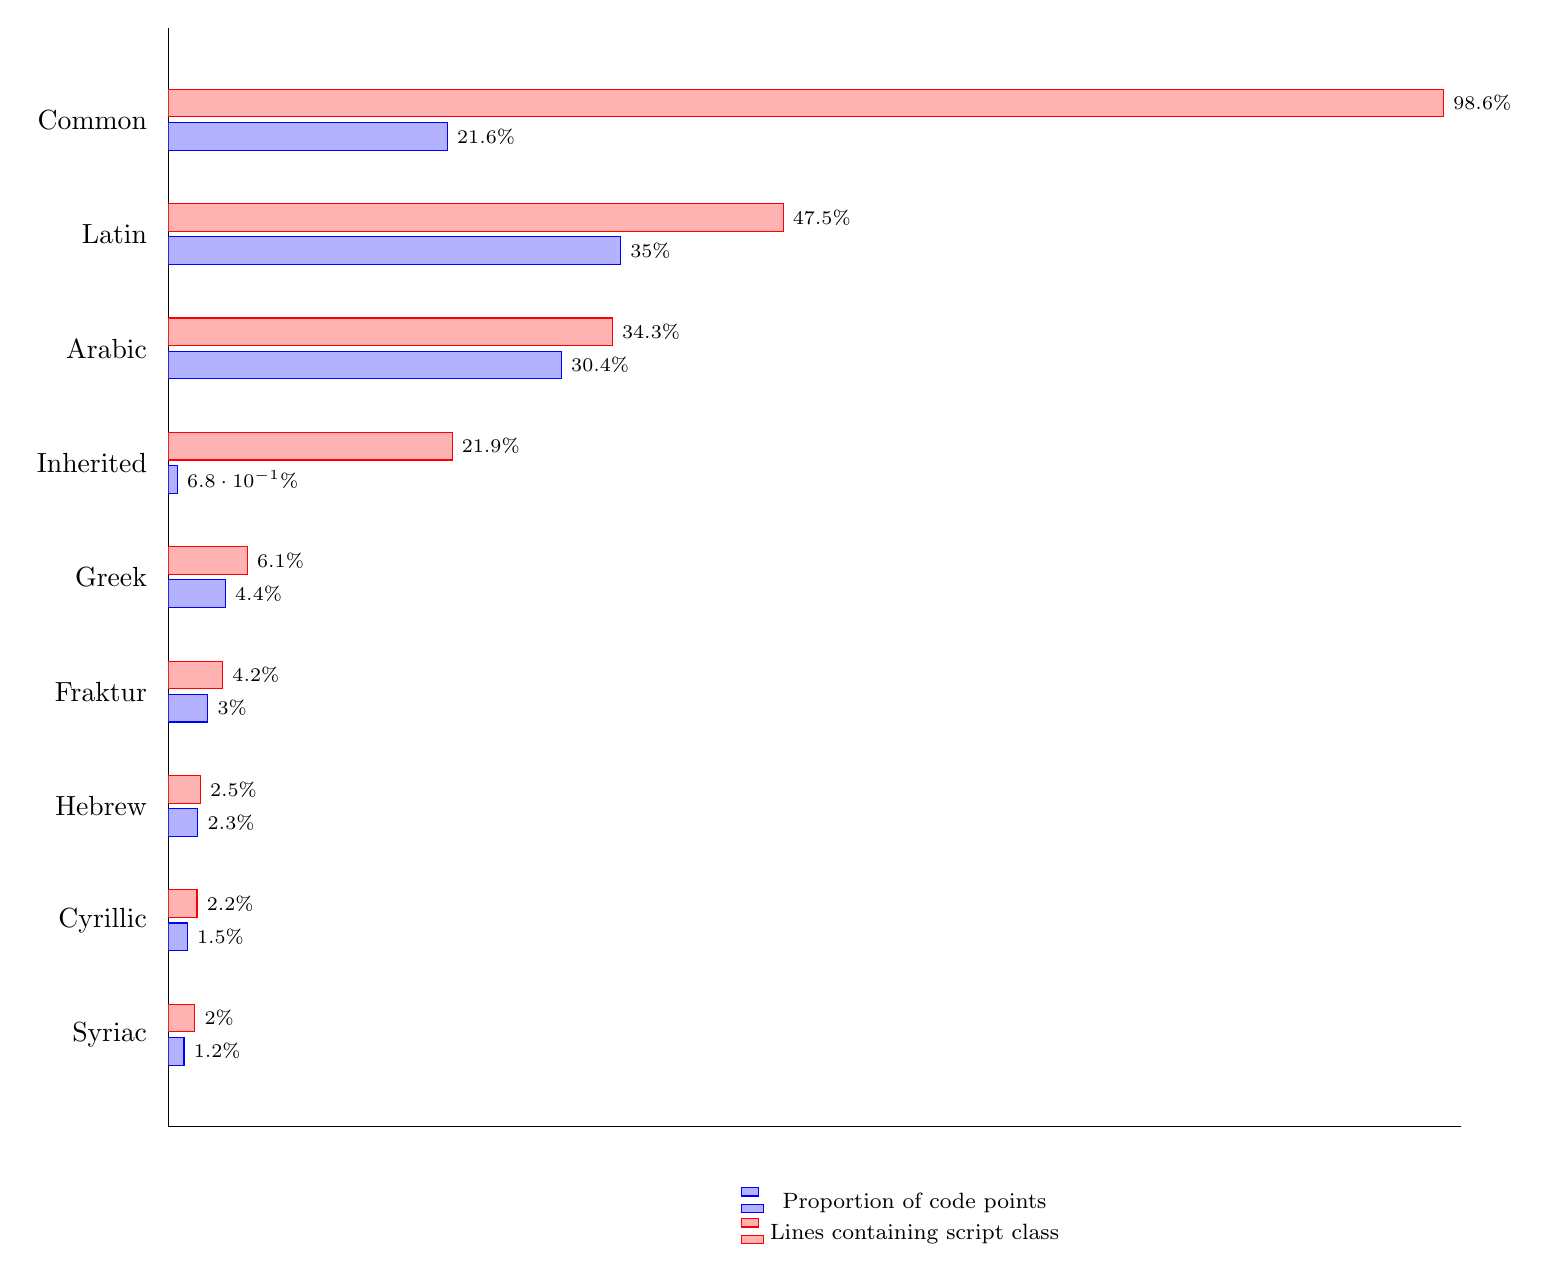
\begin{tikzpicture}
  \begin{axis}[
	axis lines*=left,
	xbar,
	width=18cm,
	xlabel={},
	xmin=0,
	xmax=1.0,
	point meta={x*100},
	ytick style={draw=none},
	xtick=\empty,
	every axis plot/.append style={fill},
	nodes near coords={\pgfmathprintnumber[precision=1]\pgfplotspointmeta\%},
	every node near coord/.append style={black, font=\scriptsize},
	nodes near coords align={horizontal},
	legend style={font=\footnotesize, draw=none, at={(0.7,-0.05)}},
	symbolic y coords={Syriac, Cyrillic, Hebrew, Fraktur, Greek, Inherited, Arabic, Latin, Common}]
	  \addplot coordinates {
		(0.3496183599324223,Latin)
		(0.30396431853540445,Arabic)
		(0.21576513077364237,Common)
		(0.04403431641055621,Greek)
		(0.030492127736907817,Fraktur)
		(0.022775620241433387,Hebrew)
		(0.014548438658383681,Cyrillic)
		(0.012010166410922564,Syriac)
		(0.006791521300327209,Inherited)
	};

	  \addplot coordinates {
		(0.4754016646187374,Latin)
		(0.34335659471866087,Arabic)
		(0.9863213780631999,Common)
		(0.06099738019613753,Greek)
		(0.04194004590452786,Fraktur)
		(0.02455196717130735,Hebrew)
		(0.022071267938701226,Cyrillic)
		(0.020309275960401548,Syriac)
		(0.21936800129830988,Inherited)
	};
	\legend{{Proportion of code points}, {Lines containing script class}}
  \end{axis}
\end{tikzpicture}
\caption{Script detection training data distribution}
\label{table:points}
\end{wrapfigure}

Emphasis recognition was evaluated on an \textbf{English and romanized Arabic
catalog on a set of 350 transcribed lines}. An additional 50 line
transcriptions were used as a test set. Overall 220 lines contain some kind of
text emphasis.

\subsection*{Script Detection}

The fully trained network yielded a \textbf{character accuracy of 94.62\%} on
the test set. Output for a French-Arabic bilingual sample page can be seen in
figure \ref{fig:high}. The misclassification of Eastern Arabic numerals as
Latin text is caused by the transcription as Latin Arabic numerals.

\subsection*{Emphasis Recognition}

The average character accuracy of the trained model over 10 runs is
\textbf{99.3\%} ($\sigma=0.16$) with \textbf{95.38\% on cursive and text with
increased spacing} ($\sigma=1.46$). When using only emphasized text accuracy as
the stopping criterium mean accuracy rises to \textbf{99.03\%} ($\sigma=0.28$).

\printbibliography

\end{multicols}
\end{document}
